\chapter{Analisi Sperimentale}
In questo capitolo verranno mostrati i risultati ottenuti applicando i due algoritmi descritti nei capitoli precedenti, Algoritmo \ref{algoritmo} e Algoritmo \ref{algoritmo2} (rispettivamente discussi nei capitoli \ref{cap 2} e \ref{cap:3}).

Verranno discusse le distribuzioni dei diversi $ k $-treelet nei differenti grafi $ G $ su cui sono state effettuate le sperimentazioni, si mostrerà come cambiano i tempi di esecuzione dei due algoritmi ed inoltre e verrà stimata laccuratezza dei risultati ottenuti rispetto a quelli calcolati per mezzo dell'algoritmo implementato in \cite{bressan2019motivo}.\\\
Per la sperimentazione sono stati utilizzati quattro differenti grafi mostrati nella tabella \ref{Tabella:grafo}, dove vi è anche una breve descrizione per ognuno.
Come si può notare i nodi e gli archi modellanno oggetti e relazioni differenti nei vari grafi  considerati, e ciò permettere di analizzare come la distribuzione dei treelet nei grafi varia a seconda del loro tipo.
Per effettuare le sperimentazioni si è fatto uso di una macchina equipaggiata di 96GiB di memoria principale e con un processore X5687 Intel(R) Xeon(R) a 3.60GHz con 256KiB di cache L1, 1MiB di cache L2
e 12 MB di cache L3.
Come è stato anche detto nei precedenti capitoli, si è sfruttato in entrambe le implementazioni il multithreading e, nello specifico, durante queste sperimentazioni si sono utilizzati 4 thread in totale.

\begin{table}
	\small
	\begin{tabular}{|p{4.4cm}|p{6cm}|p{1cm}|p{1cm}| }
		 \hline
		\multicolumn{4}{|c|}{Lista dei Grafi} \\
		\hline
		Nome del grafo & Descrizione & Nodi & Archi\\
		\hline
		\hline
		Wikipedia talk (communication) network (WiKi-Talk) \cite{leskovec2010predicting} & Grafo non orientato che indica che l'utente A e l'utente B hanno apportato modifiche sulla pagina di discussione di Wikipedia l'uno dell'altro (cioè, l'utente A ha modificato la pagina di discussione dell'utente B e viceversa). & 92000 & 360000\\
		\hline
	YeastNet \cite{babu2012interaction} & Interazioni tra membrane e proteine in ``\emph{Saccharomyces  cerevisiae}'' & 5000 & 50500\\
		\hline
		 road-luxembourg-osm \cite{bader2013graph} & Parte della rete stradale relativa alla città di Lussemburgo (non orientata) & 110000 & 120000\\
		 \hline
		 soc-Slashdot0902 \cite{leskovec2009community} &  Interazioni sociali tra utenti del sito \emph{slashdot.org}& 82000 & 870000 \\ 
		 \hline
	\end{tabular}
\caption{Tabella che descrive i diversi grafi usati nelle sperimentazioni}
\label{Tabella:grafo}
\end{table}

Per prima cosa verrà mostrata la distribuzione dei treelet nei grafi (Figure \ref{distr:1}, \ref{distr:2}, \ref{distr:3} e \ref{distr:4}).
Nello specifico per i grafi Wiki-Talk, YeastNet e road-luxembourg-osm osserveremo la distribuzione dei treelet nella tabella per $ k = 8 $, verrà limitata la visualizzazione ai 15 treelet più frequenti.
Mentre per soc-Slashdot0902 osserveremo la distribuzione dei treelet per $ k=7 $, 
 n questo caso verranno mostrati tutti poichè il numero totale di treelet distinti è $11$.
Il valore scelto per $ k $, in entrambi i casi, non rappresenta il limite raggiunto dall'esecuzione di entrambi gli algoritmi, ma semplicemente è l'ultimo valore per cui vengono prodotti valori che non superassero il limite di rappresentazione.
Questo avviene perchè il numero delle occorrenze dei treelet radicati viene rappresentato mediante interi a 64 bit, perciò per valori di $ k $ elevati tale numero supera $2^{63}-1$, il massimo intero rappresentabile in Java con il tipo di dati \emph{long}.
Nei grafici riportati di seguito le ascisse rappresentano i differenti treelet, mentre le ordinate rappresentano la frequenza dei rispettivi treelet, in percentuale.
\counterwithin*{figure}{chapter}
\renewcommand{\thefigure}{\arabic{figure}}
\begin{figure}[htbp]
	\centering
	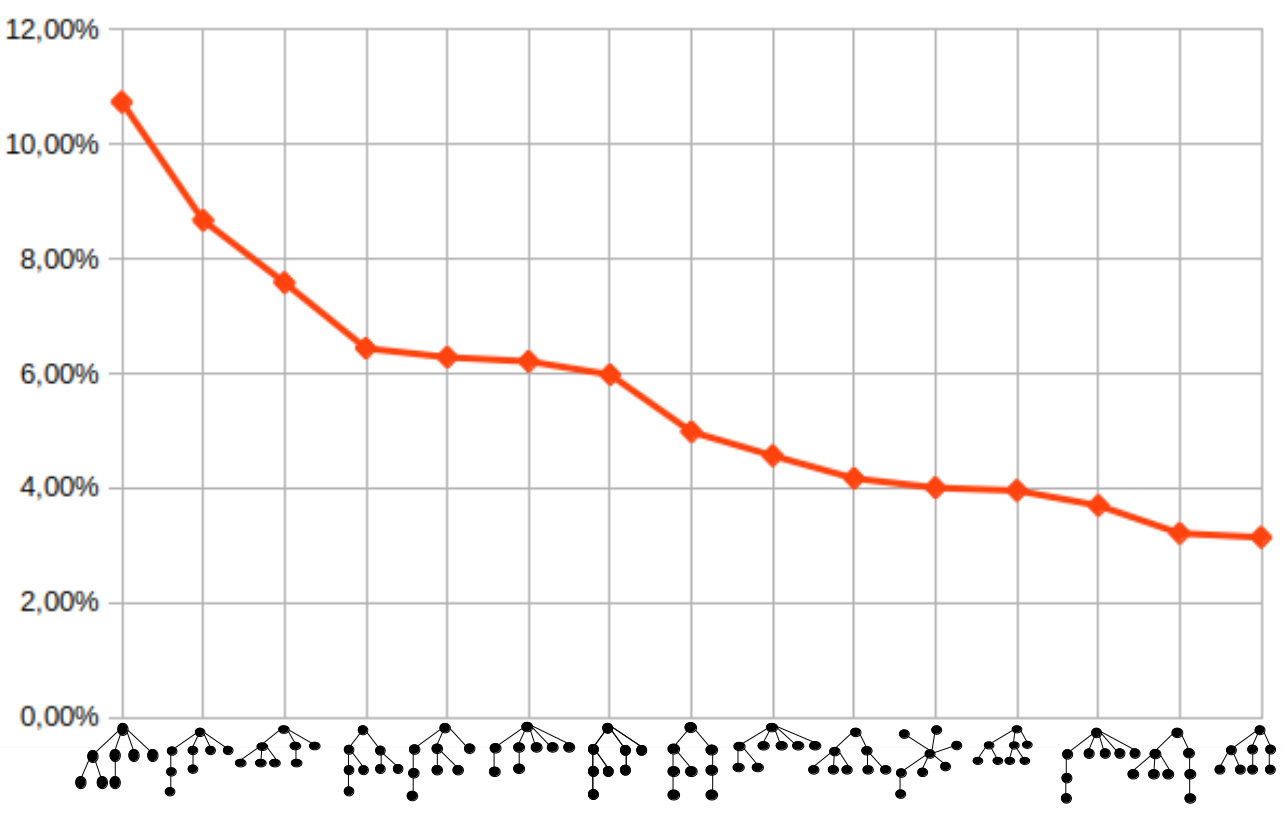
\includegraphics[width=\textwidth]{capitolo4/grafoWIKI}
		\caption{Distribuzione dei treelet con $ k=8 $ nel grafo WikiTalk}
		\label{distr:1}
\end{figure}\mbox{}
\\\\\\\\\\\\
\begin{figure}[htbp]
	\centering
	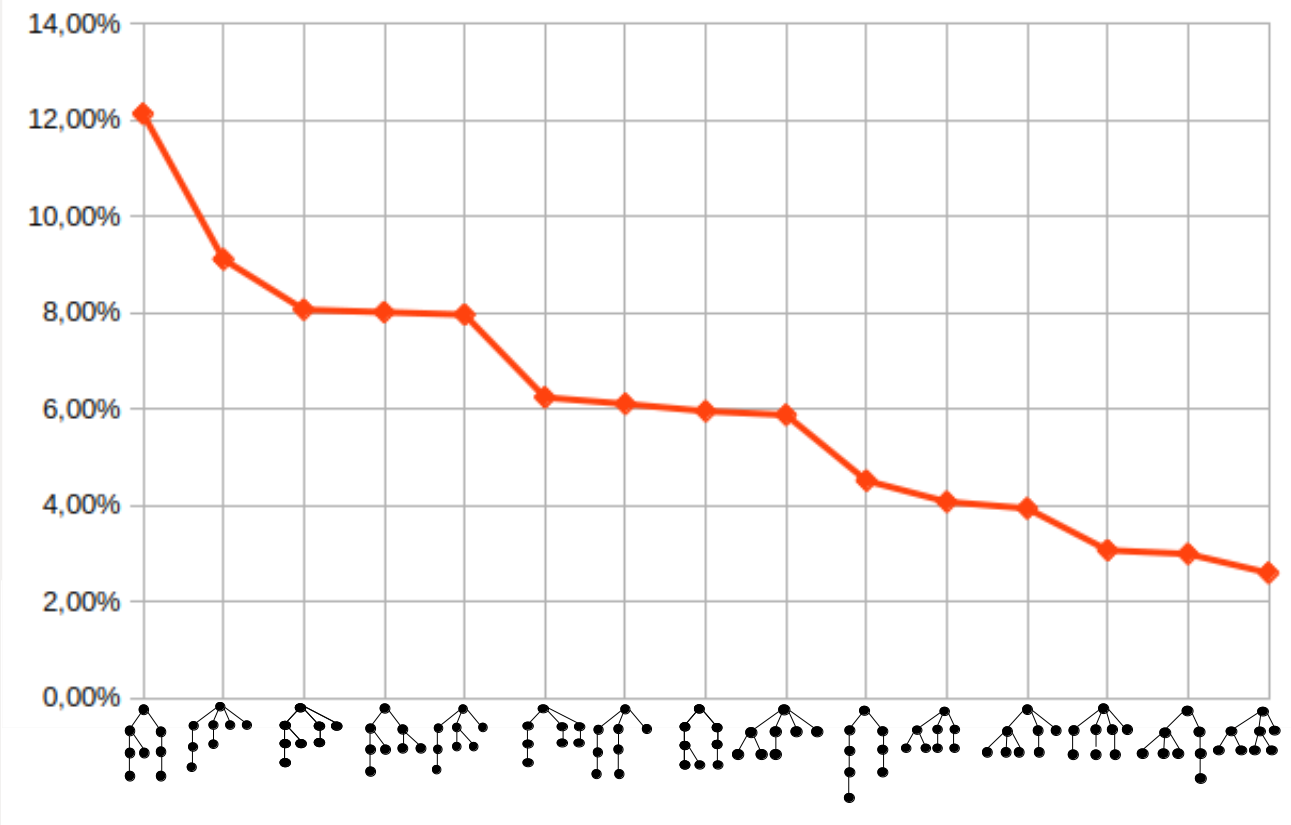
\includegraphics[width=\textwidth]{capitolo4/grafoYEAST}
	\caption{Distribuzione dei treelet con $ k=8 $ nel grafo YeastNet}
	\label{distr:2}
\end{figure}
\begin{figure}[htbp]
		\centering
	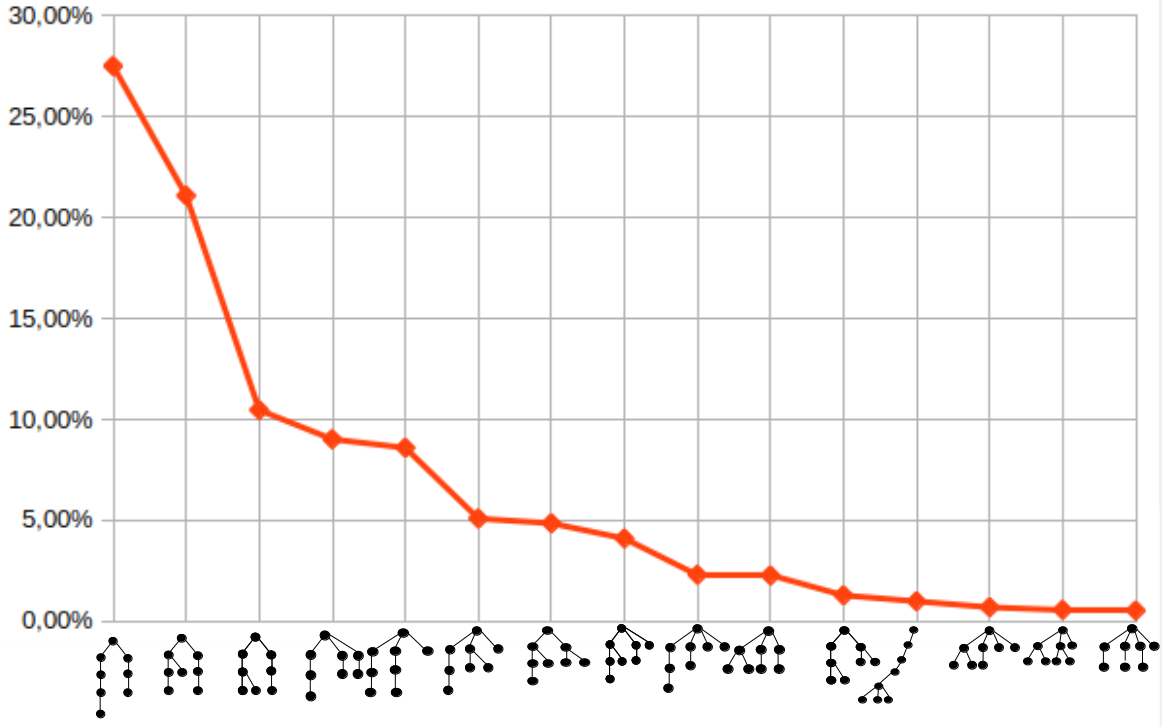
\includegraphics[width=\textwidth]{capitolo4/grafoROAD}	
		\caption{Distribuzione dei treelet con $ k=8 $ nel grafo road-luxembourg-osm }
		\label{distr:3}
\end{figure}
\begin{figure}[htbp]
		
	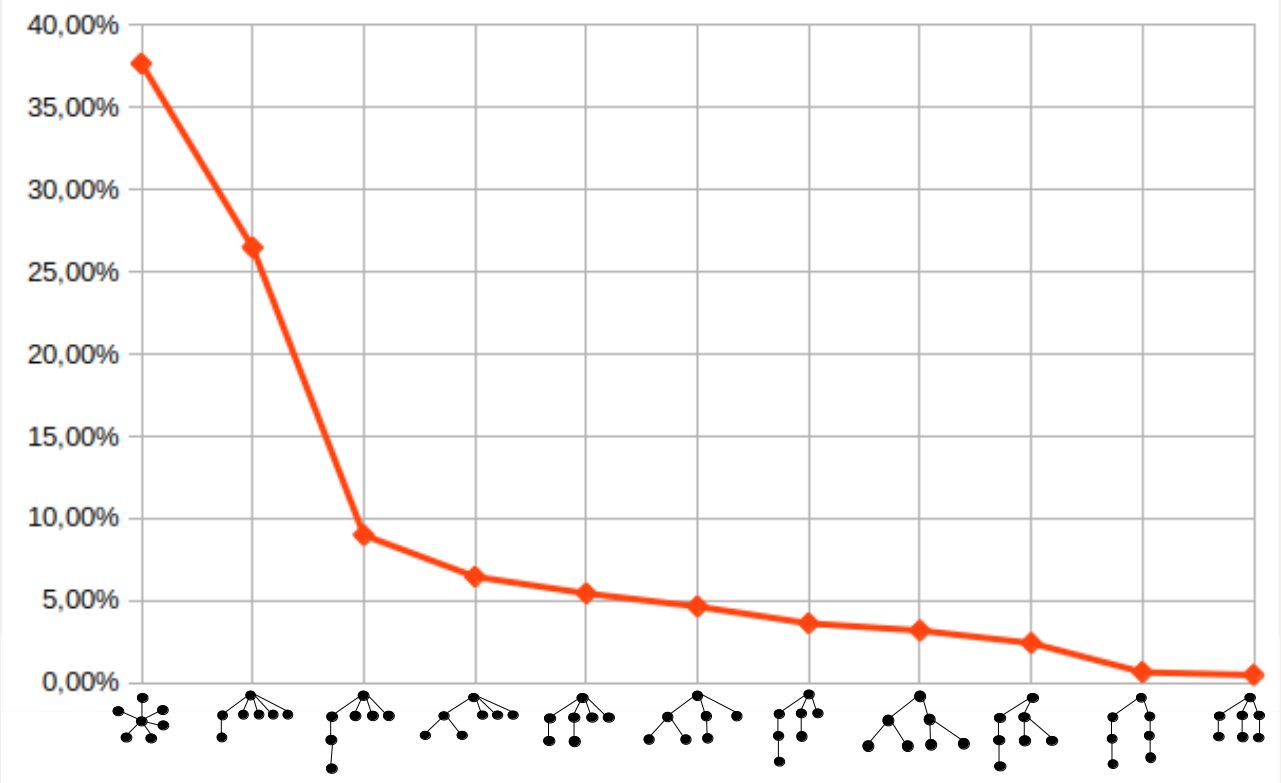
\includegraphics[width=\textwidth]{capitolo4/grafoALSH}
	\caption{Distribuzione dei treelet con $ k=7 $ nel grafo soc-Slashdot0902}
	\label{distr:4}
\end{figure}\mbox{}\\\\

Come si può notare analizzando velocemente i risultati nel grafo stradale (fig.\ref{distr:3}) e nel grafo sociale (fig.\ref{distr:4}) vi è una maggiore distribuzione di cammini e stelle, rispettivamente.
Mentre nel grafo biologico (fig.\ref{distr:2}) si possono notare strutture più complesse e maggiormente distribuite, così come nel grafo di figura \ref{distr:1}.

Un'altro aspetto interessante da vedere è come variano i tempi di esecuzione dei due algoritmi.
Nelle figure di seguito vengono mostrati, per ogni grafo e su ogni dimensione,
vengono messi a confronto i tempi di esecuzione delle due diverse implementazioni.

Come si può osservare nelle figure \ref{Tempi:1}, \ref{Tempi:2}, \ref{Tempi:3}, e \ref{Tempi:4}, l'asse delle ascisse rappresenta le diverse dimensioni dei treelet, ossia i diversi valori che $ k $ può assumere, le barre blu rappresentano i tempi relativi all'esecuzione dell'implementazione dell'Algoritmo \ref{algoritmo2} in secondi,mentre le linee rosse indicano i tempi di esecuzione relative all'esecuzione dell'implementazione dell'Algoritmo \ref{algoritmo}.
Le ordinate, dei grafi, che appunto indicano i secondi necessari per l'esecuzione, sono rappresentati in scala logaritmica.
\\

\begin{figure}[htbp]
	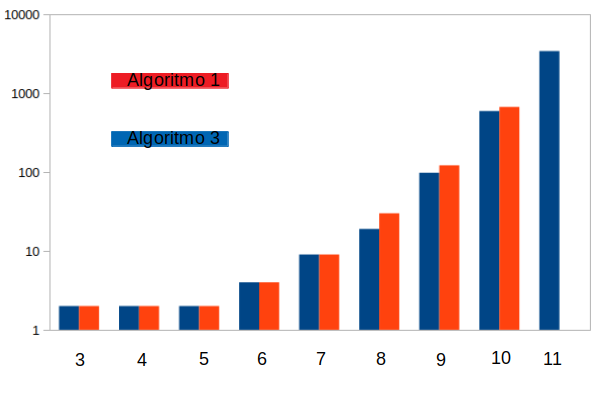
\includegraphics[width=15.4cm]{capitolo4/tempiWIKI}
	\caption{Tempi di esecuzione per gli Algoritmi \ref{algoritmo} e \ref{algoritmo2} sul grafo Wiki-Talk}
	\label{Tempi:1}
\end{figure}
\begin{figure}[htbp]
	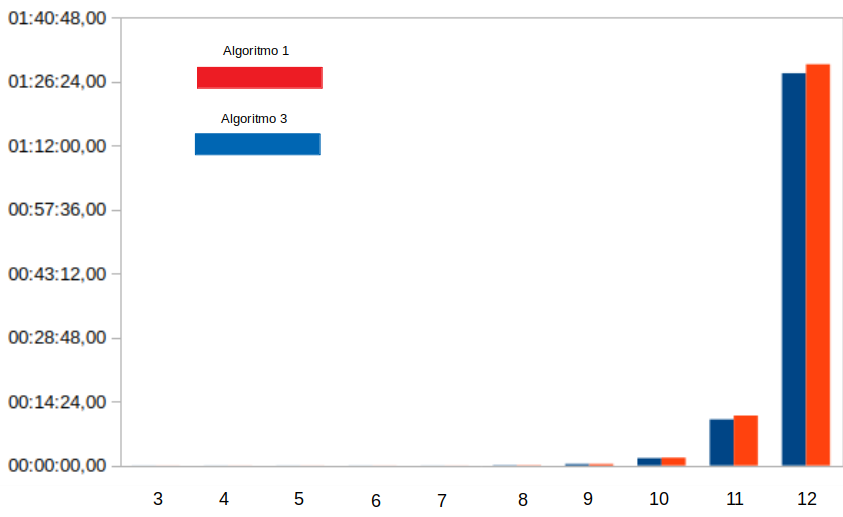
\includegraphics[width=15.4cm]{capitolo4/tempiYEAST}
	\caption{Tempi di esecuzione per gli Algoritmi \ref{algoritmo} e \ref{algoritmo2} sul grafo YeastNet}
	\label{Tempi:2}
\end{figure}
\begin{figure}[htbp]
	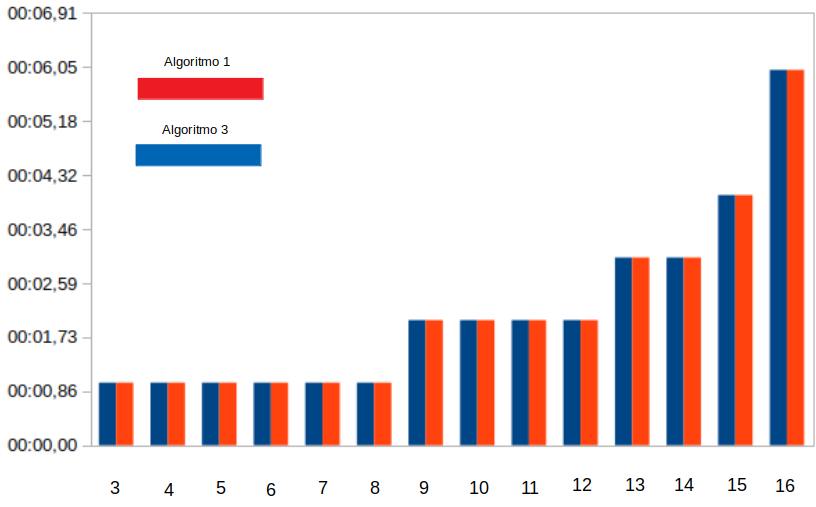
\includegraphics[width=15.4cm]{capitolo4/tempiROAD}
	\caption{Tempi di esecuzione per gli Algoritmi \ref{algoritmo} e \ref{algoritmo2} sul grafo road-luxembourg-osm}
	\label{Tempi:3}
\end{figure}
\begin{figure}[htbp]
	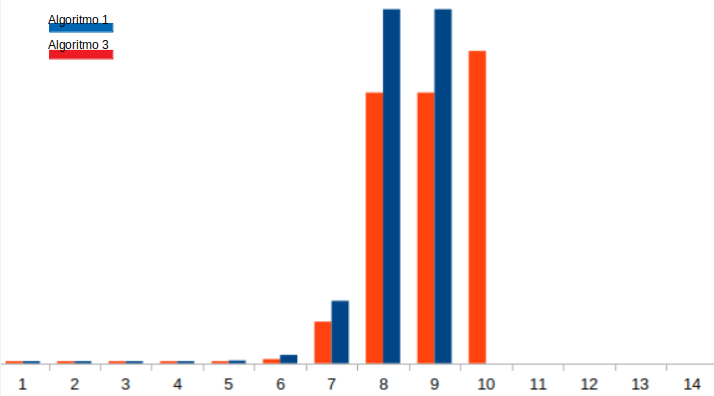
\includegraphics[width=15.4cm]{capitolo4/tempiSOC}
	\caption{Tempi di esecuzione per gli Algoritmi \ref{algoritmo} e \ref{algoritmo2} sul grafo soc-Slashdot0902}
	\label{Tempi:4}
\end{figure}

Si può notare come, in generale, i tempi di esecuzione per l'implementazione ottimizzata siano minori rispetto a quella non ottimizzata.
L'unico grafo i cui tempi restano sostanzialmente in linea è quello biologico (fig.\ref{Tempi:2}), la causa principale da attribuirsi a ciò è la dimensione ridotta del grafo. 
Infatti su grafi più grandi come ad esempio soc-Slashdot0902 (fig.\ref{Tempi:4}) la differenza si nota maggiormente. 
Un'altra cosa che si può notare vedendo i grafici, sono i differenti valori di $ k $ raggiunti: per i valori di $k$ mancanti l'esecuzione del rispettivo algoritmo è stata interrotta dopo aver raggiunto un limite sul tempo di esecuzione fissato a $2$ ore.
Per alcune combinazioni di grafi e valori di $k$, come ad esempio WikiTalk in figura \ref{Tempi:1} per $ k=11$, solo l'algoritmo~\ref{algoritmo2} ha completato la propria esecuzioni entro il tempo limite.

Per concludere l'analisi dei dati sperimentali ottenuti,
la Figura~\ref{ERROR} mostra, per il grafo YeastNet e diversi valori di $k$, la distanza in norma $1$ tra 
la distribuzione dei treelet ottenuta usando l'implemetazione dell'algoritmo~\ref{algoritmo} discussa in \cite{bressan2019motivo} e le implementazioni usate nel presente lavoro di tesi.

La distanza in norma $1$ tra le due distribuzioni è la somma delle differenze, in valore assoluti, tra le frequenze dei rispettivi treelet.
Più precisamente, se $s$ indica il numero di treelet distinti di $k$-nodi, e $f_i$ (risp. $f'_i$) indica la frequenza delle occorrenze dell'$i$-esimo treelet  conderato, come calcolata dagli gli algoritmi~\ref{algoritmo} o \ref{algoritmo2} (risp. come calcolata dall'implementazione dell'algoritmo di \cite{bressan2019motivo}), la distanza in norma $1$ è:
\[
	\sum_{i=1}^{s}{\left| f_i - f'_i \right| }.
\]


Nel grafico in figura \ref{ERROR} si mostra appunto come varia la distanza in norma $1$ all'aumentare di $ k $.\\
Sulle ascisse sono riportate le differenti dimensioni $ k $ mentre sulle ordinate si trovano la relativa distanza in noma $1$ sul grafo YeastNet.
È possibile osservare come l'errore non superi mai l'1\% in tutti i casi e come aumenti all'aumentare di $k$. 
Ciò è dovuto alla varianza intrinseca delle stime del numero di occorrenze dei treelet ottenute con la tecnica del color coding (dovute alla colorazione casuale dei nodi di $G$) e all'incremento esponenziale del numero di treelet $k$ nodi al crescere di $k$.
 

\begin{figure}[htbp]
	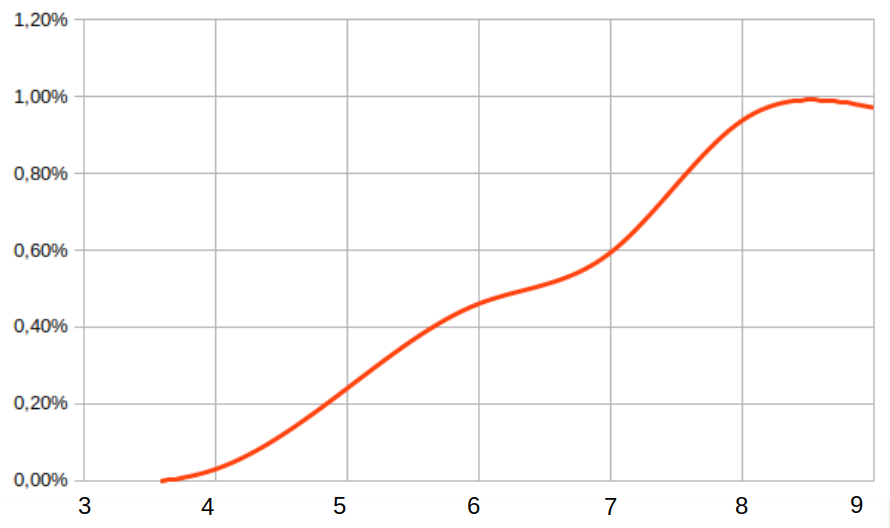
\includegraphics[width=15.4cm]{capitolo4/grafoErrorel1}
	\caption{Grafico della distanza in norma 1 sul grafo YeastNet tra la distribuzione dei treelet ottenuta con l'implementazione dell'algoritmo in \cite{bressan2019motivo} e le implementazioni usate nella presente tesi.}
	\label{ERROR}
\end{figure}


